%!TEX root = ../main.tex
\chapter{Introduzione allo studio della fisica}

\section{Le grandezze fisiche}

Concetto fondamentale al fine di affrontare lo studio dei fenomeni fisici è quello di \textbf{grandezza fisica}, termine riferito a tutte quelle proprietà di un corpo, di una sostanza o appunto di un fenomeno che possono essere misurate.
Vi sono alcune grandezze fisiche che possono essere completamente definite una volta assegnatone il valore corredato dall'unità di misura; esse per questo si dicono \emph{scalari}. Possono tuttavia sussistere casi in cui, oltre all'informazione data dal valore e dall'unità di misura, sia necessaria la specificazione di una direzione e di un verso; tali grandezze vengono chiamate \emph{vettoriali}. Ne è un esempio la forza, completamente definita dalla sua intensità, dalla sua direzione e dal suo verso.

Le unità di misura devono essere scelte in modo tale che siano facilmente riproducibili e precise. In particolare modo, il più diffuso sistema di unità di misura, noto come \textbf{Sistema Internazionale}, SI, definisce sette grandezze fisiche fondamentali dalle quali, sfruttando le leggi fisiche che le legano, possono essere ricavate tutte le altre grandezze. Esse sono riportate in seguito:

\begin{center}
	\begin{tabular}{lll}
	\toprule
	Grandezza & Unità di misura &Simbolo \\
	\midrule
	lunghezza & metri & $m$ \\
	massa  & chilogrammi & $kg$ \\
	tempo & secondi  & $s$\\
	temperatura &gradi kelvin & $K$\\
	quantità di materia &moli  & $mol$\\
	intensità luminosa  &candele& $cd$ \\
	intensità di corrente elettrica  &ampère & $A$ \\
	\bottomrule
	\end{tabular}
\end{center}

\paragraph{Osservazione} Le equazioni fisiche sono omogenee dal punto di vista dimensionale, ciò significa che in un'equazione l'unità di misura è la stessa sia a sinistra che a destra.

\section{Introduzione al calcolo vettoriale}

\subsection{Definizione di un vettore e delle sue componenti}

Il \textbf{vettore} è l'ente matematico adatto alla rappresentazione delle grandezze vettoriali precedentemente definite e per le quali vale un'algebra che differisce da quella scalare.

\begin{figure}[htpb]
	\centering

	\tikzset{every picture/.style={line width=0.75pt}} %set default line width to 0.75pt

	\begin{tikzpicture}[x=0.75pt,y=0.75pt,yscale=-1,xscale=1]
	%uncomment if require: \path (0,300); %set diagram left start at 0, and has height of 300

	%Straight Lines [id:da4464327382646005]
	\draw  [dash pattern={on 0.84pt off 2.51pt}]  (300,80) -- (120,190) ;
	%Straight Lines [id:da6798121572011886]
	\draw [line width=1.5]    (170,160) -- (246.61,112.12) ;
	\draw [shift={(250,110)}, rotate = 507.99] [fill={rgb, 255:red, 0; green, 0; blue, 0 }  ][line width=0.08]  [draw opacity=0] (13.4,-6.43) -- (0,0) -- (13.4,6.44) -- (8.9,0) -- cycle    ;

	% Text Node
	\draw (197,121) node    {$\vec{v}$};
	% Text Node
	\draw (222.5,156.5) node    {$\vec{u}_v$};

	\end{tikzpicture}
\end{figure}

Matematicamente un vettore ha infinite rappresentazioni: infatti tutti i segmenti orientati di eguale lunghezza, paralleli ed equiversi sono rappresentazioni dello stesso vettore e quindi equivalenti, si dice che essi formano un sistema di vettori \textbf{equipollenti}. Fissata una direzione orientata $\vec{r}$ vi sono infiniti vettori che hanno quella direzione e differiscono solo nel modulo e nel verso. In particolare fra di essi esiste un vettore $\vec{u}$ che è concorde in verso a $\vec{r}$ e ha modulo unitario:

\[
	\vec{v}=\abs{\vec{v}} \,\vec{u}_v \qquad \text{dove $\vec{v}=$ modulo del vettore $\vec{v}$}
\]

Più in generale, un qualsiasi vettore di modulo unitario si definisce \textbf{versore}.

Si consideri il sistema di riferimento cartesiano: esso può essere rappresentato dai versori $\vec{u}_x$, $\vec{u}_y$, $\vec{u}_z$.

\begin{figure}[htpb]
	\centering

	\tikzset{every picture/.style={line width=0.75pt}} %set default line width to 0.75pt        

	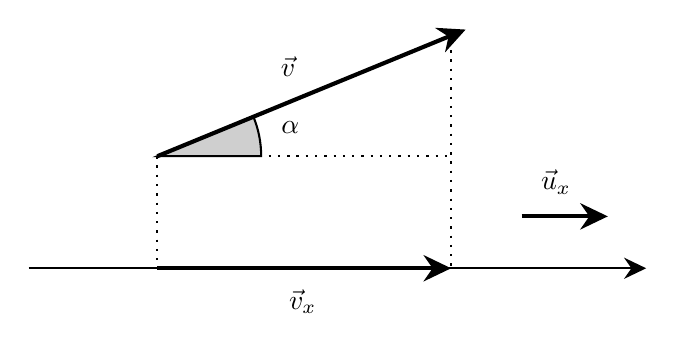
\begin{tikzpicture}[x=0.75pt,y=0.75pt,yscale=-1,xscale=1]
	%uncomment if require: \path (0,300); %set diagram left start at 0, and has height of 300

	%Shape: Pie [id:dp6201472441222928] 
	\draw  [fill={rgb, 255:red, 207; green, 207; blue, 207 }  ,fill opacity=1 ] (219.17,91.78) .. controls (221.64,97.7) and (223,104.19) .. (223,111) -- (173,111) -- cycle ;
	%Straight Lines [id:da5356624891507755] 
	\draw    (111,165) -- (405.5,165) ;
	\draw [shift={(408.5,165)}, rotate = 180] [fill={rgb, 255:red, 0; green, 0; blue, 0 }  ][line width=0.08]  [draw opacity=0] (10.72,-5.15) -- (0,0) -- (10.72,5.15) -- (7.12,0) -- cycle    ;
	%Straight Lines [id:da993433031949847] 
	\draw [line width=1.5]    (173,111) -- (317.8,51.52) ;
	\draw [shift={(321.5,50)}, rotate = 517.6700000000001] [fill={rgb, 255:red, 0; green, 0; blue, 0 }  ][line width=0.08]  [draw opacity=0] (13.4,-6.43) -- (0,0) -- (13.4,6.44) -- (8.9,0) -- cycle    ;
	%Straight Lines [id:da38435392810852576] 
	\draw  [dash pattern={on 0.84pt off 2.51pt}]  (173,111) -- (314.5,111) ;
	%Straight Lines [id:da6456289887316091] 
	\draw  [dash pattern={on 0.84pt off 2.51pt}]  (173,111) -- (173,165) ;
	%Straight Lines [id:da4993284795246429] 
	\draw  [dash pattern={on 0.84pt off 2.51pt}]  (314.5,51) -- (314.5,165) ;
	%Straight Lines [id:da9011995931714469] 
	\draw [line width=1.5]    (173,165) -- (310.5,165) ;
	\draw [shift={(314.5,165)}, rotate = 180] [fill={rgb, 255:red, 0; green, 0; blue, 0 }  ][line width=0.08]  [draw opacity=0] (13.4,-6.43) -- (0,0) -- (13.4,6.44) -- (8.9,0) -- cycle    ;
	%Straight Lines [id:da693284506691856] 
	\draw [line width=1.5]    (348.5,140) -- (386,140) ;
	\draw [shift={(390,140)}, rotate = 180] [fill={rgb, 255:red, 0; green, 0; blue, 0 }  ][line width=0.08]  [draw opacity=0] (13.4,-6.43) -- (0,0) -- (13.4,6.44) -- (8.9,0) -- cycle    ;

	% Text Node
	\draw (236,68) node    {$\vec{v}$};
	% Text Node
	\draw (237,97) node    {$\alpha $};
	% Text Node
	\draw (243,181) node    {$\vec{v}_{x}$};
	% Text Node
	\draw (365,123.5) node    {$\vec{u}_{x}$};

	\end{tikzpicture}
\end{figure}

Proiettare un qualunque vettore $\vec{v}$ su uno dei tre assi significa andare a valutare quanto vale $\vec{v}$ lungo di esso e la quantità risultante dalla proiezione è detta \emph{componente} del vettore $\vec{v}$ lungo il suddetto asse. Ad esempio, per quanto riguarda l'asse $x$, essa è data da:

\[
	\vec{v}_x=v\cos\alpha\, \vec{u}_x
\]

Ovviamente l'espressione è analoga considerando l'asse delle $y$ o delle $z$.

\begin{figure}[htpb]
	\centering

	\tikzset{every picture/.style={line width=0.75pt}} %set default line width to 0.75pt

	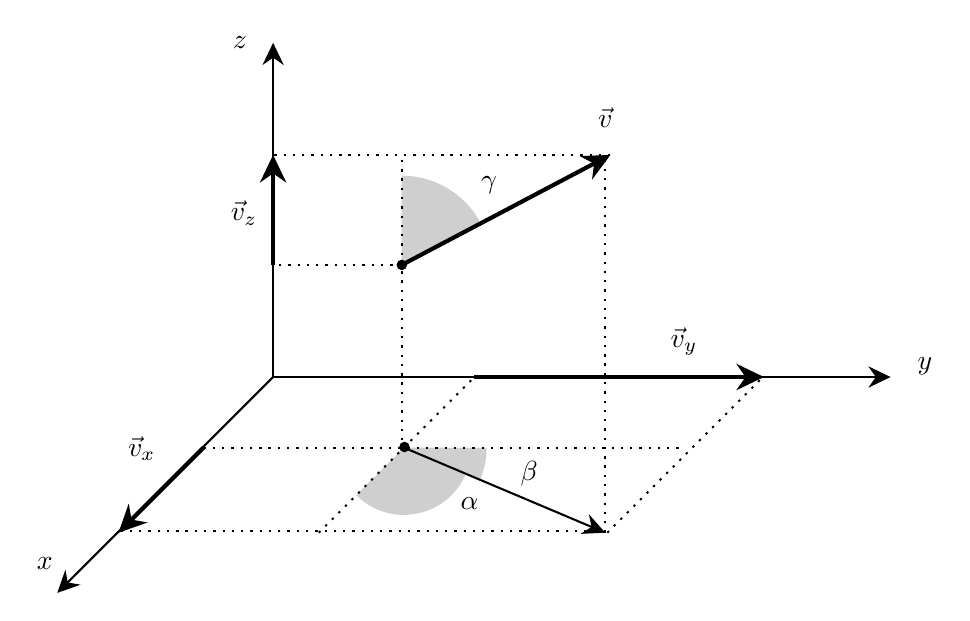
\begin{tikzpicture}[x=0.75pt,y=0.75pt,yscale=-1,xscale=1]
	%uncomment if require: \path (0,339); %set diagram left start at 0, and has height of 339

	%Shape: Pie [id:dp9667084827284058]
	\draw  [draw opacity=0][fill={rgb, 255:red, 207; green, 207; blue, 207 }  ,fill opacity=1 ] (253.86,219.15) .. controls (253.84,224.43) and (252.79,229.47) .. (250.91,234.08) -- (214,219) -- cycle ;
	%Shape: Pie [id:dp8404828655017231]
	\draw  [draw opacity=0][fill={rgb, 255:red, 207; green, 207; blue, 207 }  ,fill opacity=1 ] (243.79,231.84) .. controls (238.81,243.36) and (227.35,251.43) .. (214,251.43) .. controls (205.05,251.43) and (196.94,247.8) .. (191.07,241.93) -- (214,219) -- cycle ;
	%Shape: Pie [id:dp1921798512080477]
	\draw  [draw opacity=0][fill={rgb, 255:red, 207; green, 207; blue, 207 }  ,fill opacity=1 ] (212.88,88) .. controls (212.92,88) and (212.96,88) .. (213,88) .. controls (229.58,88) and (243.97,97.38) .. (251.14,111.13) -- (213,131) -- cycle ;
	%Straight Lines [id:da40010362980616754]
	\draw    (151,185) -- (445.5,185) ;
	\draw [shift={(448.5,185)}, rotate = 180] [fill={rgb, 255:red, 0; green, 0; blue, 0 }  ][line width=0.08]  [draw opacity=0] (10.72,-5.15) -- (0,0) -- (10.72,5.15) -- (7.12,0) -- cycle    ;
	%Straight Lines [id:da7488969456901324]
	\draw [line width=1.5]    (213,131) -- (309.96,79.87) ;
	\draw [shift={(313.5,78)}, rotate = 512.19] [fill={rgb, 255:red, 0; green, 0; blue, 0 }  ][line width=0.08]  [draw opacity=0] (13.4,-6.43) -- (0,0) -- (13.4,6.44) -- (8.9,0) -- cycle    ;
	%Straight Lines [id:da6439329921032626]
	\draw  [dash pattern={on 0.84pt off 2.51pt}]  (313.5,78) -- (150.5,78) ;
	%Straight Lines [id:da06318067450836828]
	\draw    (151,185) -- (151,27) ;
	\draw [shift={(151,24)}, rotate = 450] [fill={rgb, 255:red, 0; green, 0; blue, 0 }  ][line width=0.08]  [draw opacity=0] (10.72,-5.15) -- (0,0) -- (10.72,5.15) -- (7.12,0) -- cycle    ;
	%Straight Lines [id:da3735738788431415]
	\draw    (151,185) -- (49.12,286.88) ;
	\draw [shift={(47,289)}, rotate = 315] [fill={rgb, 255:red, 0; green, 0; blue, 0 }  ][line width=0.08]  [draw opacity=0] (10.72,-5.15) -- (0,0) -- (10.72,5.15) -- (7.12,0) -- cycle    ;
	%Straight Lines [id:da4212922877969385]
	\draw  [dash pattern={on 0.84pt off 2.51pt}]  (213,220) -- (213,78) ;
	%Straight Lines [id:da8129583034692129]
	\draw  [dash pattern={on 0.84pt off 2.51pt}]  (173,260) -- (248,185) ;
	%Straight Lines [id:da5309983983054607]
	\draw  [dash pattern={on 0.84pt off 2.51pt}]  (117.5,219) -- (348,219) ;
	%Straight Lines [id:da3180503246327162]
	\draw [line width=0.75]    (214,219) -- (308.24,258.83) ;
	\draw [shift={(311,260)}, rotate = 202.91] [fill={rgb, 255:red, 0; green, 0; blue, 0 }  ][line width=0.08]  [draw opacity=0] (10.72,-5.15) -- (0,0) -- (10.72,5.15) -- (7.12,0) -- cycle    ;
	%Straight Lines [id:da4455044711565159]
	\draw  [dash pattern={on 0.84pt off 2.51pt}]  (311,260) -- (311,79) ;
	%Straight Lines [id:da26365916114812626]
	\draw  [dash pattern={on 0.84pt off 2.51pt}]  (312,260) -- (387,185) ;
	%Straight Lines [id:da02453639685058273]
	\draw  [dash pattern={on 0.84pt off 2.51pt}]  (77.5,259) -- (308,259) ;
	%Straight Lines [id:da9177326517219728]
	\draw  [dash pattern={on 0.84pt off 2.51pt}]  (213,131) -- (151,131) ;
	%Straight Lines [id:da8000425396378845]
	\draw [line width=1.5]    (248,185) -- (383.5,185) ;
	\draw [shift={(387.5,185)}, rotate = 180] [fill={rgb, 255:red, 0; green, 0; blue, 0 }  ][line width=0.08]  [draw opacity=0] (13.4,-6.43) -- (0,0) -- (13.4,6.44) -- (8.9,0) -- cycle    ;
	%Straight Lines [id:da135170186754614]
	\draw [line width=1.5]    (117.5,219) -- (79.33,257.17) ;
	\draw [shift={(76.5,260)}, rotate = 315] [fill={rgb, 255:red, 0; green, 0; blue, 0 }  ][line width=0.08]  [draw opacity=0] (13.4,-6.43) -- (0,0) -- (13.4,6.44) -- (8.9,0) -- cycle    ;
	%Straight Lines [id:da5870054208298388]
	\draw [line width=1.5]    (151,131) -- (151,82) ;
	\draw [shift={(151,78)}, rotate = 450] [fill={rgb, 255:red, 0; green, 0; blue, 0 }  ][line width=0.08]  [draw opacity=0] (13.4,-6.43) -- (0,0) -- (13.4,6.44) -- (8.9,0) -- cycle    ;
	%Shape: Circle [id:dp2419013582112337]
	\draw  [fill={rgb, 255:red, 0; green, 0; blue, 0 }  ,fill opacity=1 ] (212.29,218.71) .. controls (212.29,217.61) and (213.18,216.71) .. (214.29,216.71) .. controls (215.39,216.71) and (216.29,217.61) .. (216.29,218.71) .. controls (216.29,219.82) and (215.39,220.71) .. (214.29,220.71) .. controls (213.18,220.71) and (212.29,219.82) .. (212.29,218.71) -- cycle ;
	%Shape: Circle [id:dp012579141877352207]
	\draw  [fill={rgb, 255:red, 0; green, 0; blue, 0 }  ,fill opacity=1 ] (211,131) .. controls (211,129.9) and (211.9,129) .. (213,129) .. controls (214.1,129) and (215,129.9) .. (215,131) .. controls (215,132.1) and (214.1,133) .. (213,133) .. controls (211.9,133) and (211,132.1) .. (211,131) -- cycle ;

	% Text Node
	\draw (311,60) node    {$\vec{v}$};
	% Text Node
	\draw (41,275) node    {$x$};
	% Text Node
	\draw (135,24) node    {$z$};
	% Text Node
	\draw (137,106) node    {$\vec{v}_z$};
	% Text Node
	\draw (87.67,219.33) node    {$\vec{v}_x$};
	% Text Node
	\draw (349,168) node    {$\vec{v}_y$};
	% Text Node
	\draw (255,92.67) node    {$\gamma $};
	% Text Node
	\draw (245.67,246) node    {$\alpha $};
	% Text Node
	\draw (274.33,231.33) node    {$\beta $};
	% Text Node
	\draw (465,180) node    {$y$};

	\end{tikzpicture}
\end{figure}

\subsection{Operazioni fra vettori}

\paragraph{Prodotto di un vettore per uno scalare} Il risultato è un vettore che ha la stessa direzione del vettore di partenza $\vec{v}$, modulo pari a $\abs{\vec{v}}$ moltiplicato per lo scalare $m$, stesso verso di $\vec{v}$ se $m>0$, opposto se $m<0$.

\[
	\vec{v}\,m
\]

\paragraph{Somma vettoriale} Dati due vettori $\vec{a}$ e $\vec{b}$ la somma è un vettore che si ottiene graficamente tramite il cosiddetto \emph{metodo del parallelogramma}: si applica nell'origine di $\vec{a}$ anche il vettore $\vec{b}$ spostandolo parallelamente a se stesso; il vettore somma coincide con la diagonale del parallelogramma che ha come lati $\vec{a}$ e $\vec{b}$.

\begin{figure}[htpb]
	\centering
		

	\tikzset{every picture/.style={line width=0.75pt}} %set default line width to 0.75pt

	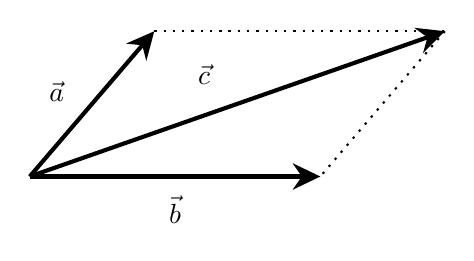
\begin{tikzpicture}[x=0.75pt,y=0.75pt,yscale=-1,xscale=1]
	%uncomment if require: \path (0,300); %set diagram left start at 0, and has height of 300

	%Straight Lines [id:da2440730162800544]
	\draw [line width=1.5]    (160,180) -- (296,180) ;
	\draw [shift={(300,180)}, rotate = 180] [fill={rgb, 255:red, 0; green, 0; blue, 0 }  ][line width=0.08]  [draw opacity=0] (13.4,-6.43) -- (0,0) -- (13.4,6.44) -- (8.9,0) -- cycle    ;
	%Straight Lines [id:da4892608957102378]
	\draw [line width=1.5]    (160,180) -- (217.4,113.04) ;
	\draw [shift={(220,110)}, rotate = 490.6] [fill={rgb, 255:red, 0; green, 0; blue, 0 }  ][line width=0.08]  [draw opacity=0] (13.4,-6.43) -- (0,0) -- (13.4,6.44) -- (8.9,0) -- cycle    ;
	%Straight Lines [id:da3719981116584463]
	\draw  [dash pattern={on 0.84pt off 2.51pt}]  (220,110) -- (360,110) ;
	%Straight Lines [id:da6616324461946157]
	\draw  [dash pattern={on 0.84pt off 2.51pt}]  (360,110) -- (300,180) ;
	%Straight Lines [id:da8126730528636246]
	\draw [line width=1.5]    (160,180) -- (356.22,111.32) ;
	\draw [shift={(360,110)}, rotate = 520.71] [fill={rgb, 255:red, 0; green, 0; blue, 0 }  ][line width=0.08]  [draw opacity=0] (13.4,-6.43) -- (0,0) -- (13.4,6.44) -- (8.9,0) -- cycle    ;

	% Text Node
	\draw (173,139) node    {$\vec{a}$};
	% Text Node
	\draw (230,196) node    {$\vec{b}$};
	% Text Node
	\draw (244,131) node    {$\vec{c}$};

	\end{tikzpicture}
\end{figure}

Riprendendo il concetto di scomposizione dei vettori sugli assi cartesiani, si osservi che, dal momento che i tre versori $\vec{u}_x, \vec{u}_y, \vec{u}_z$ sono mutuamente ortogonali fra di loro:

\[
	\vec{v}=\vec{v}_x + \vec{v}_y + \vec{v}_z
\]

Questo permette di affermare che le operazioni fra vettori possono essere eseguite più facilmente sfruttandone la scomposizione lungo gli assi cartesiani. Il vettore somma infatti ha come componenti la somma delle componenti dei singoli vettori di partenza.
È infine evidente che il risultato della somma di più vettori non dipende dal loro ordine: vale la \emph{proprietà associativa}.

\paragraph{Differenza fra due vettori} Tale operazione può essere facilmente definita come la somma fra il primo vettore e l'opposto del secondo, ossia il secondo moltiplicato per $-1$.
\\
\\
\\
\\
Si definiscono inoltre due diverse operazioni di prodotto che danno rispettivamente come risultato una quantità scalare o vettoriale.

\paragraph{Prodotto scalare} Dati due vettori $\vec{a}$ e $\vec{b}$ si definisce prodotto scalare la quantità:

\[
	\vec{a}\cdot \vec{b}= \abs{\vec{a}}\abs{\vec{b}}\cos\alpha
\]

Indicando con $\alpha$ l'angolo formato dai due vettori, il risultato del prodotto scalare è una quantità scalare data dal prodotto dei moduli di $\vec{a}$ e di $\vec{b}$ per il coseno dell'angolo fra di essi compreso. Tale quantità è anche pari alla somma dei prodotti delle componenti omologhe dei singoli vettori. Il prodotto scalare è nullo non solo se uno dei due vettori è nullo, ma anche se essi sono ortogonali. Valgono inoltre le proprietà associativa e distributiva. Un altro modo, fisicamente molto significativo, di rappresentare il prodotto scalare è il seguente:

\[
	\vec{a}\cdot \vec{b}= \abs{\vec{a}}\,(\abs{\vec{b}}\cos\alpha)
\]

\begin{figure}[htpb]
	\centering

	\tikzset{every picture/.style={line width=0.75pt}} %set default line width to 0.75pt        

	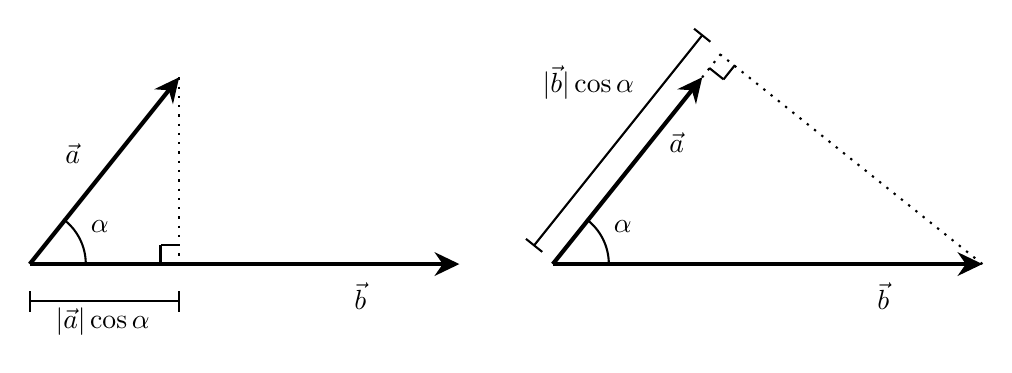
\begin{tikzpicture}[x=0.75pt,y=0.75pt,yscale=-0.9,xscale=0.9]
	%uncomment if require: \path (0,300); %set diagram left start at 0, and has height of 300

	%Straight Lines [id:da27354838547691696] 
	\draw [line width=1.5]    (60,180) -- (286,180) ;
	\draw [shift={(290,180)}, rotate = 180] [fill={rgb, 255:red, 0; green, 0; blue, 0 }  ][line width=0.08]  [draw opacity=0] (13.4,-6.43) -- (0,0) -- (13.4,6.44) -- (8.9,0) -- cycle    ;
	%Straight Lines [id:da5678151431421725] 
	\draw [line width=1.5]    (60,180) -- (137.5,83.12) ;
	\draw [shift={(140,80)}, rotate = 488.66] [fill={rgb, 255:red, 0; green, 0; blue, 0 }  ][line width=0.08]  [draw opacity=0] (13.4,-6.43) -- (0,0) -- (13.4,6.44) -- (8.9,0) -- cycle    ;
	%Straight Lines [id:da3953822489943375] 
	\draw  [dash pattern={on 0.84pt off 2.51pt}]  (140,80) -- (140,180) ;
	%Shape: Arc [id:dp8373824492896644] 
	\draw  [draw opacity=0] (77.98,155.98) .. controls (85.28,161.46) and (90,170.18) .. (90,180) .. controls (90,180.2) and (90,180.41) .. (89.99,180.61) -- (60,180) -- cycle ; \draw   (77.98,155.98) .. controls (85.28,161.46) and (90,170.18) .. (90,180) .. controls (90,180.2) and (90,180.41) .. (89.99,180.61) ;
	%Straight Lines [id:da9058029829917178] 
	\draw    (130,170) -- (130,180) ;
	%Straight Lines [id:da715168339128929] 
	\draw    (140,170) -- (130,170) ;
	%Straight Lines [id:da4600264437767905] 
	\draw    (140,200) -- (60,200) ;
	\draw [shift={(60,200)}, rotate = 360] [color={rgb, 255:red, 0; green, 0; blue, 0 }  ][line width=0.75]    (0,5.59) -- (0,-5.59)   ;
	\draw [shift={(140,200)}, rotate = 360] [color={rgb, 255:red, 0; green, 0; blue, 0 }  ][line width=0.75]    (0,5.59) -- (0,-5.59)   ;
	%Straight Lines [id:da9351143374864943] 
	\draw [line width=1.5]    (340,180) -- (566,180) ;
	\draw [shift={(570,180)}, rotate = 180] [fill={rgb, 255:red, 0; green, 0; blue, 0 }  ][line width=0.08]  [draw opacity=0] (13.4,-6.43) -- (0,0) -- (13.4,6.44) -- (8.9,0) -- cycle    ;
	%Straight Lines [id:da5952375166706461] 
	\draw [line width=1.5]    (340,180) -- (417.5,83.12) ;
	\draw [shift={(420,80)}, rotate = 488.66] [fill={rgb, 255:red, 0; green, 0; blue, 0 }  ][line width=0.08]  [draw opacity=0] (13.4,-6.43) -- (0,0) -- (13.4,6.44) -- (8.9,0) -- cycle    ;
	%Straight Lines [id:da15985064204341093] 
	\draw  [dash pattern={on 0.84pt off 2.51pt}]  (430,67.5) -- (340,180) ;
	%Shape: Arc [id:dp6036328273138647] 
	\draw  [draw opacity=0] (357.98,155.98) .. controls (365.28,161.46) and (370,170.18) .. (370,180) .. controls (370,180.2) and (370,180.41) .. (369.99,180.61) -- (340,180) -- cycle ; \draw   (357.98,155.98) .. controls (365.28,161.46) and (370,170.18) .. (370,180) .. controls (370,180.2) and (370,180.41) .. (369.99,180.61) ;
	%Straight Lines [id:da17422970123026738] 
	\draw  [dash pattern={on 0.84pt off 2.51pt}]  (570,180) -- (430,68) ;
	%Straight Lines [id:da09367412711699274] 
	\draw    (437.5,73.5) -- (431.4,81.13) ;
	%Straight Lines [id:da7293699633872541] 
	\draw    (431.4,81.13) -- (423.78,75.03) ;

	%Straight Lines [id:da22095363277223878] 
	\draw    (420,57.5) -- (330,170) ;
	\draw [shift={(330,170)}, rotate = 308.65999999999997] [color={rgb, 255:red, 0; green, 0; blue, 0 }  ][line width=0.75]    (0,5.59) -- (0,-5.59)   ;
	\draw [shift={(420,57.5)}, rotate = 308.65999999999997] [color={rgb, 255:red, 0; green, 0; blue, 0 }  ][line width=0.75]    (0,5.59) -- (0,-5.59)   ;

	% Text Node
	\draw (83,121) node    {$\vec{a}$};
	% Text Node
	\draw (237,197) node    {$\vec{b}$};
	% Text Node
	\draw (99,211) node    {$|\vec{a} |\cos \alpha $};
	% Text Node
	\draw (97.5,160) node    {$\alpha $};
	% Text Node
	\draw (406.33,115) node    {$\vec{a}$};
	% Text Node
	\draw (517,197) node    {$\vec{b}$};
	% Text Node
	\draw (359,83) node    {$|\vec{b} |\cos \alpha $};
	% Text Node
	\draw (377.5,160) node    {$\alpha $};

	\end{tikzpicture}
\end{figure}
\FloatBarrier
Ossia: il prodotto scalare fra due vettori è eguale al prodotto del modulo di uno dei vettori per la proiezione su di esso dell'altro vettore.

\paragraph{Prodotto vettoriale} Dati due vettori $\vec{a}$ e $\vec{b}$ si definisce prodotto vettoriale il vettore $\vec{c}$, che si indica con il simbolo:

\[
	\vec{c}=\vec{a} \times \vec{b}
\]

Tale espressione si legge `\textit{a vettor b}'. Esso ha:

\begin{itemize}
	\item direzione perpendicolare al piano individuato da $\vec{a}$ e $\vec{b}$;
	\item verso di una normale vite destrogira (ruotando da $\vec{a}$ a $\vec{b}$ nel verso di una vite il verso di $\vec{c}$ è indicato dalla punta della vite);
	\item modulo pari a $\abs{\vec{a}}\abs{\vec{b}}\sin\alpha$ che coincide con l'area del parallelogramma di lati $\vec{a}$ e $\vec{b}$.
\end{itemize}

\begin{figure}[htpb]
	\centering

	% Pattern Info
	 
	\tikzset{
	pattern size/.store in=\mcSize, 
	pattern size = 5pt,
	pattern thickness/.store in=\mcThickness, 
	pattern thickness = 0.3pt,
	pattern radius/.store in=\mcRadius, 
	pattern radius = 1pt}
	\makeatletter
	\pgfutil@ifundefined{pgf@pattern@name@_uar2b48nb}{
	\pgfdeclarepatternformonly[\mcThickness,\mcSize]{_uar2b48nb}
	{\pgfqpoint{0pt}{-\mcThickness}}
	{\pgfpoint{\mcSize}{\mcSize}}
	{\pgfpoint{\mcSize}{\mcSize}}
	{
	\pgfsetcolor{\tikz@pattern@color}
	\pgfsetlinewidth{\mcThickness}
	\pgfpathmoveto{\pgfqpoint{0pt}{\mcSize}}
	\pgfpathlineto{\pgfpoint{\mcSize+\mcThickness}{-\mcThickness}}
	\pgfusepath{stroke}
	}}
	\makeatother
	\tikzset{every picture/.style={line width=0.75pt}} %set default line width to 0.75pt        

	\begin{tikzpicture}[x=0.75pt,y=0.75pt,yscale=-1,xscale=1]
	%uncomment if require: \path (0,300); %set diagram left start at 0, and has height of 300

	%Shape: Parallelogram [id:dp4647818089148623] 
	\draw  [draw opacity=0][pattern=_uar2b48nb,pattern size=3.75pt,pattern thickness=0.75pt,pattern radius=0pt, pattern color={rgb, 255:red, 222; green, 222; blue, 222}] (170,120) -- (310,120) -- (250,190) -- (110,190) -- cycle ;
	%Straight Lines [id:da07829591594899687] 
	\draw [line width=1.5]    (110,190) -- (246,190) ;
	\draw [shift={(250,190)}, rotate = 180] [fill={rgb, 255:red, 0; green, 0; blue, 0 }  ][line width=0.08]  [draw opacity=0] (13.4,-6.43) -- (0,0) -- (13.4,6.44) -- (8.9,0) -- cycle    ;
	%Straight Lines [id:da3908497787206091] 
	\draw [line width=1.5]    (110,190) -- (167.4,123.04) ;
	\draw [shift={(170,120)}, rotate = 490.6] [fill={rgb, 255:red, 0; green, 0; blue, 0 }  ][line width=0.08]  [draw opacity=0] (13.4,-6.43) -- (0,0) -- (13.4,6.44) -- (8.9,0) -- cycle    ;
	%Straight Lines [id:da5010366366593619] 
	\draw  [dash pattern={on 0.84pt off 2.51pt}]  (170,120) -- (310,120) ;
	%Straight Lines [id:da3791967059336212] 
	\draw  [dash pattern={on 0.84pt off 2.51pt}]  (310,120) -- (250,190) ;
	%Straight Lines [id:da18657789312970685] 
	\draw [line width=1.5]    (110,190) -- (110,44) ;
	\draw [shift={(110,40)}, rotate = 450] [fill={rgb, 255:red, 0; green, 0; blue, 0 }  ][line width=0.08]  [draw opacity=0] (13.4,-6.43) -- (0,0) -- (13.4,6.44) -- (8.9,0) -- cycle    ;
	%Shape: Arc [id:dp11097324545322373] 
	\draw  [draw opacity=0] (124.11,172.11) .. controls (133.57,175.14) and (140,181.12) .. (140,188) .. controls (140,188.4) and (139.98,188.79) .. (139.94,189.18) -- (110,188) -- cycle ; \draw   (124.11,172.11) .. controls (133.57,175.14) and (140,181.12) .. (140,188) .. controls (140,188.4) and (139.98,188.79) .. (139.94,189.18) ;
	%Shape: Free Drawing [id:dp43190093896936044] 
	\draw  [color={rgb, 255:red, 0; green, 0; blue, 0 }  ,draw opacity=1 ][line width=1.5] [line join = round][line cap = round] (497,53.5) .. controls (497,58.51) and (495.62,63.5) .. (496,68.5) .. controls (497.03,81.92) and (514.53,115.3) .. (524,125.5) .. controls (531.26,133.32) and (540.84,142.34) .. (547,148.5) .. controls (549.31,150.81) and (562.21,153.29) .. (561,154.5) ;
	%Shape: Free Drawing [id:dp2469297143503948] 
	\draw  [color={rgb, 255:red, 0; green, 0; blue, 0 }  ,draw opacity=1 ][line width=1.5] [line join = round][line cap = round] (497,53.5) .. controls (495.57,53.5) and (492.53,50.05) .. (490,51.5) .. controls (469.32,63.32) and (495.46,100.04) .. (482,113.5) .. controls (476.53,118.97) and (465.75,113.42) .. (460,111.5) .. controls (445.65,106.72) and (410.75,96.13) .. (398,102.5) .. controls (390.34,106.33) and (400.23,113.34) .. (406,115.5) .. controls (415.9,119.21) and (443.5,123.76) .. (447,132.5) .. controls (448.96,137.41) and (436.2,141.66) .. (432,142.5) .. controls (419.35,145.03) and (406.92,147.84) .. (409,164.5) .. controls (409.34,167.2) and (420.48,166.55) .. (421,166.5) .. controls (423.36,166.29) and (428.74,162.13) .. (430,161.5) .. controls (436.52,158.24) and (447.08,156.5) .. (454,156.5) ;
	%Shape: Free Drawing [id:dp2699755526754224] 
	\draw  [color={rgb, 255:red, 0; green, 0; blue, 0 }  ,draw opacity=1 ][line width=1.5] [line join = round][line cap = round] (458,157.5) .. controls (458,160.85) and (456.4,164.2) .. (457,167.5) .. controls (459.38,180.58) and (481.86,171.69) .. (489,170.5) .. controls (495.92,169.35) and (499.73,168.13) .. (505,165.5) .. controls (505.3,165.35) and (505.92,165.82) .. (506,165.5) .. controls (508.11,157.07) and (479.9,156.93) .. (473,156.5) .. controls (467.31,156.14) and (460.03,154.47) .. (456,158.5) ;
	%Shape: Free Drawing [id:dp0065945962483409115] 
	\draw  [color={rgb, 255:red, 0; green, 0; blue, 0 }  ,draw opacity=1 ][line width=1.5] [line join = round][line cap = round] (461,178.5) .. controls (461,199.46) and (482.17,191.41) .. (496,184.5) .. controls (499.72,182.64) and (510.02,180.44) .. (511,176.5) .. controls (512.56,170.28) and (506.23,170.5) .. (502,170.5) ;
	%Shape: Free Drawing [id:dp7784500736262567] 
	\draw  [color={rgb, 255:red, 0; green, 0; blue, 0 }  ,draw opacity=1 ][line width=1.5] [line join = round][line cap = round] (477,192.5) .. controls (490.14,201.26) and (503.9,194.34) .. (519,195.5) .. controls (529.05,196.27) and (536.53,209.5) .. (547,209.5) ;
	%Shape: Free Drawing [id:dp5945113146611334] 
	\draw  [color={rgb, 255:red, 155; green, 155; blue, 155 }  ,draw opacity=1 ][line width=1.5] [line join = round][line cap = round] (489,81.5) .. controls (490.8,81.5) and (492.73,80.77) .. (494,79.5) ;
	%Shape: Free Drawing [id:dp863292993267458] 
	\draw  [color={rgb, 255:red, 155; green, 155; blue, 155 }  ,draw opacity=1 ][line width=1.5] [line join = round][line cap = round] (407,111.5) .. controls (408.41,108.69) and (409.78,105.72) .. (412,103.5) ;
	%Shape: Free Drawing [id:dp8451572197613626] 
	\draw  [color={rgb, 255:red, 155; green, 155; blue, 155 }  ,draw opacity=1 ][line width=1.5] [line join = round][line cap = round] (428,117.5) .. controls (428,114.67) and (428.82,110.5) .. (432,110.5) ;
	%Shape: Free Drawing [id:dp5382674395061409] 
	\draw  [color={rgb, 255:red, 155; green, 155; blue, 155 }  ,draw opacity=1 ][line width=1.5] [line join = round][line cap = round] (445,126.5) .. controls (446.87,119.94) and (447.46,118.04) .. (452,113.5) ;
	%Shape: Free Drawing [id:dp887365066791401] 
	\draw  [color={rgb, 255:red, 155; green, 155; blue, 155 }  ,draw opacity=1 ][line width=1.5] [line join = round][line cap = round] (425,151.5) .. controls (426.75,154.41) and (427,158.1) .. (427,161.5) ;
	%Shape: Free Drawing [id:dp773009858564268] 
	\draw  [color={rgb, 255:red, 155; green, 155; blue, 155 }  ,draw opacity=1 ][line width=1.5] [line join = round][line cap = round] (436,146.5) .. controls (437.63,149.21) and (439,152.34) .. (439,155.5) ;
	%Shape: Free Drawing [id:dp4112761415080526] 
	\draw  [color={rgb, 255:red, 155; green, 155; blue, 155 }  ,draw opacity=1 ][line width=1.5] [line join = round][line cap = round] (448,142.5) .. controls (450.79,142.5) and (451.66,151.84) .. (450,153.5) ;
	%Shape: Free Drawing [id:dp6484449716929179] 
	\draw  [color={rgb, 255:red, 155; green, 155; blue, 155 }  ,draw opacity=1 ][line width=1.5] [line join = round][line cap = round] (454,136.5) .. controls (460.79,136.5) and (474,145.82) .. (474,153.5) ;
	%Shape: Free Drawing [id:dp6067471895852834] 
	\draw  [color={rgb, 255:red, 155; green, 155; blue, 155 }  ,draw opacity=1 ][line width=1.5] [line join = round][line cap = round] (479,120.5) .. controls (476.4,123.1) and (478,127.82) .. (478,131.5) ;
	%Shape: Free Drawing [id:dp3287032141639632] 
	\draw  [color={rgb, 255:red, 155; green, 155; blue, 155 }  ,draw opacity=1 ][line width=1.5] [line join = round][line cap = round] (485,123.5) .. controls (485,134.19) and (492.94,147.06) .. (502,152.5) ;
	%Shape: Free Drawing [id:dp2903477573462456] 
	\draw  [color={rgb, 255:red, 155; green, 155; blue, 155 }  ,draw opacity=1 ][line width=1.5] [line join = round][line cap = round] (528,145.5) .. controls (528,149.96) and (527.22,152.39) .. (523,154.5) ;
	%Shape: Free Drawing [id:dp21087767721795547] 
	\draw  [color={rgb, 255:red, 155; green, 155; blue, 155 }  ,draw opacity=1 ][line width=1.5] [line join = round][line cap = round] (524,185.5) .. controls (524,180.61) and (532,160.97) .. (532,158.5) ;
	%Shape: Free Drawing [id:dp7518276869665781] 
	\draw  [color={rgb, 255:red, 155; green, 155; blue, 155 }  ,draw opacity=1 ][line width=1.5] [line join = round][line cap = round] (470,161.5) .. controls (470,166.13) and (471,167.93) .. (471,171.5) ;
	%Shape: Free Drawing [id:dp4308694134358355] 
	\draw  [color={rgb, 255:red, 155; green, 155; blue, 155 }  ,draw opacity=1 ][line width=1.5] [line join = round][line cap = round] (485,160.5) .. controls (485,164.02) and (486,165.61) .. (486,168.5) ;
	%Shape: Free Drawing [id:dp03487892767445544] 
	\draw  [color={rgb, 255:red, 155; green, 155; blue, 155 }  ,draw opacity=1 ][line width=1.5] [line join = round][line cap = round] (474,179.5) .. controls (474.62,181.96) and (475.59,184.39) .. (477,186.5) ;
	%Shape: Free Drawing [id:dp7220964275690744] 
	\draw  [color={rgb, 255:red, 155; green, 155; blue, 155 }  ,draw opacity=1 ][line width=1.5] [line join = round][line cap = round] (489,175.5) .. controls (489,177.68) and (489.72,182.5) .. (492,182.5) ;

	%Straight Lines [id:da980106951249955] 
	\draw [line width=1.5]    (405,107) -- (368.79,94.78) ;
	\draw [shift={(365,93.5)}, rotate = 378.65] [fill={rgb, 255:red, 0; green, 0; blue, 0 }  ][line width=0.08]  [draw opacity=0] (13.4,-6.43) -- (0,0) -- (13.4,6.44) -- (8.9,0) -- cycle    ;
	%Straight Lines [id:da9191850982532173] 
	\draw [line width=1.5]    (416,159) -- (384.54,175.63) ;
	\draw [shift={(381,177.5)}, rotate = 332.14] [fill={rgb, 255:red, 0; green, 0; blue, 0 }  ][line width=0.08]  [draw opacity=0] (13.4,-6.43) -- (0,0) -- (13.4,6.44) -- (8.9,0) -- cycle    ;
	%Straight Lines [id:da5262132613493635] 
	\draw [line width=1.5]    (489,64) -- (489,30.5) ;
	\draw [shift={(489,26.5)}, rotate = 450] [fill={rgb, 255:red, 0; green, 0; blue, 0 }  ][line width=0.08]  [draw opacity=0] (13.4,-6.43) -- (0,0) -- (13.4,6.44) -- (8.9,0) -- cycle    ;

	% Text Node
	\draw (147,121) node    {$\vec{b}$};
	% Text Node
	\draw (213,207) node    {$\vec{a}$};
	% Text Node
	\draw (154.5,57) node    {$\vec{c} =\vec{a} \times \vec{b}$};
	% Text Node
	\draw (216.5,148) node   [align=left] {area = $\displaystyle |\vec{c} |$};
	% Text Node
	\draw (147.5,170) node    {$\alpha $};
	% Text Node
	\draw (375,75) node    {$\vec{a}$};
	% Text Node
	\draw (378,157) node    {$\vec{b}$};
	% Text Node
	\draw (518.5,28) node    {$\vec{a} \times \vec{b}$};

	\end{tikzpicture}
\end{figure}
\FloatBarrier
È bene osservare che il prodotto vettoriale non gode della proprietà commutativa. Infatti eseguendo il prodotto $\vec{b}\times \vec{a}$ si ottiene il vettore $-\vec{c}$, opposto a $\vec{c}$. Si dice dunque che il prodotto vettoriale è \emph{anticommutativo}. Esso può essere iterato, ma va specificato l'ordine delle diverse operazioni, perché non vale la proprietà associativa.

Calcolare il prodotto vettoriale $\vec{a} \times \vec{b}$ equivale a calcolare il determinante della seguente matrice:

\[
	\begin{bmatrix}
		\vec{u}_x & \vec{u}_y & \vec{u}_z \\
		a_x & a_y & a_z \\
		b_x & b_y & b_z
	\end{bmatrix}
\]

Ossia

\[
	\vec{a} \times \vec{b} = (a_y b_z - a_z b_y)\vec{u}_x + (a_z b_x - a_x b_z) \vec{u}_y + (a_x b_y - a_y b_x) \vec{u}_z
\]